\section{Experiments}
\label{sec:experiments}
\label{sec:usecases}

We evaluate the algorithm of Section~\ref{sec:solution} on query-refinement pairs and on consistent-query-answering (CQA) pairs.
The experiments answer five questions:
\begin{itemize}[leftmargin=*,itemsep=1pt,topsep=2pt]
  \item[\textbf{(E1)}] How insightful and interesting are the explanations we release? We check whether they tell an analyst something about the difference between $Q_1$ and $Q_2$ that the two queries and the constraint do not already say (Section~\ref{sec:usecase-results}).
  \item[\textbf{(E2)}] What is the effect of the privacy budget $\epsilon$ on the quality of the released explanations, measured against the baselines $\Bone$--$\Bthree$ (Section~\ref{subsec:quality})?
  \item[\textbf{(E3)}] What is the effect of the query pair, through the gap between its leading candidates, and of the smoothing constant $\gamma$ on accuracy (Section~\ref{subsec:quality})?
  \item[\textbf{(E4)}] What is the effect of the data size $N$, the number of explanations $k$, the number of kept views $\tau$ and the budget $\epsilon$ on running time (Section~\ref{subsec:scalability})?
  \item[\textbf{(E5)}] What does privacy cost in running time, compared with the non-private baselines (Section~\ref{subsec:scalability})?
\end{itemize}
Section~\ref{subsec:exp-setup} describes the baselines, the datasets, the query pairs and the default parameters.

% ---------------------------------------------------------------
\subsection{Experiment Setup}
\label{subsec:exp-setup}

\paragraph{Baselines.}
No prior system explains the difference of two query outputs privately, so, as in DPXplain, we compare against reference points that each remove one ingredient of the algorithm.
All baselines are measured against Definition~\ref{def:setobj}: the set-level objective $F_\lambda$ with the unsmoothed $\HD$ ($\gamma_{\mathrm{eval}}=0$).
The mechanism uses smoothing to control noise, so using it in the metric as well would make the comparison circular.
We report the ApproxRatio, the score of the released set divided by the score of the baseline's set.
\begin{itemize}[leftmargin=*,itemsep=1pt,topsep=2pt]
  \item \textbf{\Bone{} ($\epsilon\to\infty$).} The same algorithm with the noise made negligible. The ratio to \Bone{} is the cost of noise alone, with the architecture held fixed.
  \item \textbf{\Btwo{} (exhaustive optimum).} Scores every size-$k$ subset of candidates with $F_\lambda$ and returns the best one, non-privately. The full space ($\binom{350}{5}\approx5\times10^{11}$) cannot be enumerated, but the optimum can be computed exactly on the top-$k$ candidates of each attribute: a set that used a candidate outside the top $k$ of its attribute could swap in an unused candidate with a higher score without lowering $F_\lambda$. This leaves $50$ candidates and $\binom{50}{5}\approx2.1\times10^{6}$ subsets.
  \item \textbf{\Bthree{} (non-private greedy).} Keeps the top-$\tau$ views by $\Use$ and then picks $k$ explanations greedily, with no noise anywhere.
\end{itemize}
\Btwo{} and \Bthree{} differ from the private algorithm in two ways at once (no noise and no private view filter), so the gap to them is the total cost of privacy. The gap to \Bone{} is the part due to noise.

\paragraph{Datasets.}
We use four datasets.
Numeric attributes are bucketed into six quantile bins, and views are conjunctions of at most two atomic conditions ($\ell\le2$).
\begin{itemize}[leftmargin=*,itemsep=1pt,topsep=2pt]
  \item \textbf{Adult.} The UCI census extract, $N=48{,}842$ tuples, with demographic and employment attributes (education, occupation, hours per week, marital status, race, gender) and a binary income flag. It is a standard dataset in fairness-aware data management, which makes it a natural source of representation constraints.
  \item \textbf{Tax.} The synthetic tax benchmark used in the data-cleaning literature, $N=500{,}000$ tuples, with attributes such as state, marital status, number of children, salary and tax rate. We use it to test a dataset roughly ten times larger than Adult.
  \item \textbf{StackOverflow.} The Developer Survey, with attributes such as years of professional coding, remote-work status, company size, country, languages and AI-tool usage. We use it for contrasts between two subpopulations.
  \alon{TODO: fill in $N$ and the number of explanation attributes for StackOverflow, and state which survey year is used. Everything in the repository for this dataset, and for IPUMS-CPS, was produced on a synthetic generator, not on the downloaded survey, so no StackOverflow number below may be quoted until it is re-run on the real file.}
  \item \textbf{Hospital.} The hospital-records dataset from the repair literature~\cite{rekatsinas2017}, which violates the functional dependencies $\texttt{HospitalName}\rightarrow\texttt{ZipCode}$, $\texttt{HospitalName}\rightarrow\texttt{PhoneNumber}$ and $\texttt{ZipCode}\rightarrow\texttt{City}$. It is the only dataset with integrity violations, so it is the one we use for CQA.
\end{itemize}

\paragraph{Query pairs.}
Table~\ref{tab:query-pairs} lists the twelve pairs, three per dataset. They come from three sources.
\begin{itemize}[leftmargin=*,itemsep=1pt,topsep=2pt]
  \item \emph{Query refinement (A1--A3, T1--T3).} In every refinement pair $Q$ violates a representation constraint, and the refined query $Q'$ is the query returned by running the ERICA algorithm~\cite{LMSJ23,ERICA} on $Q$ and that constraint. The pairs are therefore the output of a refinement system and not hand-picked contrasts.
  \item \emph{Consistent query answering (H1--H3).} $Q$ is a selection query on Hospital and $Q_\Sigma$ is its consistent answer (Definition~\ref{def:consistent-answer}). We compute $Q_\Sigma(D)$ with the conflict-hypergraph algorithm~\cite{chomicki2004}: a conflict is a set of tuples that jointly violate a dependency, and for a selection query the consistent answer is $Q(D)$ without the tuples that belong to some conflict. Section~\ref{subsec:case-cqa} explains why this pair is worth explaining.
  \item \emph{Contrasts (S1--S3).} The StackOverflow pairs compare two subpopulations rather than a query and its refinement. They test the framework when the two outputs are far apart.
\end{itemize}

\begin{table*}[t]
\centering
\small
\caption{The twelve query pairs. Shares are on the real data. Cells marked TBD are not available in the repository and need a run. In H1--H3, $Q_\Sigma$ is the consistent answer of $Q$.}
\label{tab:query-pairs}
\begin{tabular}{@{}llp{4.6cm}p{4.6cm}l@{}}
\toprule
ID & Data & $Q$ & $Q'$ (or $Q_\Sigma$) & Constraint (share $Q\rightarrow Q'$)\\
\midrule
A1 & Adult & \texttt{occupation='Craft-repair' AND hours$\ge$40} & \texttt{hours$\ge$40} & $\ge25\%$ female ($4.7\%\rightarrow26.9\%$)\\
A2 & Adult & \texttt{education IN (Bachelors, Masters) AND hours$\ge$50} & \texttt{education=Masters AND hours$\ge$30} & $\ge25\%$ female ($19.5\%\rightarrow30.6\%$)\\
A3 & Adult & TBD & TBD & TBD\\
T1 & Tax & \texttt{MaritalStatus='M' AND Rate$\le$5} & \texttt{Rate$\le$5} & $\ge30\%$ HasChild ($3.5\%\rightarrow50.1\%$)\\
T2 & Tax & TBD & TBD & TBD\\
T3 & Tax & TBD & TBD & TBD\\
S1 & StackOv. & \texttt{YearsCodePro$\ge$10} & \texttt{YearsCodePro$<$4} & contrast\\
S2 & StackOv. & \texttt{WorkRemote='Fully remote'} & \texttt{WorkRemote='On-site'} & contrast\\
S3 & StackOv. & \texttt{JobSat$>$5 AND UsingAI='Yes'} & \texttt{JobSat$>$5 AND UsingAI='No'} & contrast\\
H1 & Hospital & \texttt{HospitalType='Acute Care Hospitals'} & $Q_\Sigma$ & 3 FDs (TBD)\\
H2 & Hospital & TBD (selection on \texttt{EmergencyService}) & $Q_\Sigma$ & 3 FDs (TBD)\\
H3 & Hospital & TBD (selection on \texttt{HospitalOwner}) & $Q_\Sigma$ & 3 FDs (TBD)\\
\bottomrule
\end{tabular}
\end{table*}

\alon{Check that A1 is the pair the earlier drafts called ``Adult 6.7'' (the real counts match a craft-repair, full-time query, but the repository only keeps the label). T1 was called ``Tax 6.6''. A3, T2 and T3 do not exist in the repository as real-data runs; pick them so that each dataset has one pair whose result is surprising and one where the explanation is a sanity check. For A3, T2, T3 run ERICA on the chosen $Q$ and constraint and record the refined query it returns.}
\alon{H1--H3: the Hospital file was not available in the environment this draft was written in, so the three pairs are defined by a rule and still need a run. Take every single-predicate selection on \texttt{HospitalType}, \texttt{EmergencyService} and \texttt{HospitalOwner}, compute $Q_\Sigma$ with the conflict-hypergraph algorithm, and keep, for each attribute, the selection in which $Q_\Sigma$ drops between $10\%$ and $90\%$ of $Q$ and the dropped tuples are spread unevenly over the other attributes. Fill in the exact predicates and the counts.}

\paragraph{Default parameters.}
Unless stated otherwise: $k=5$ explanations, diversity $\lambda=0.5$, total budget $\epsilon=1$ split equally between view selection, explanation selection and histogram release, $\tau=\min(3k,|\mathcal P|)=15$ views kept by the first stage, and $\gamma=2\ln(\tau|\Attrs|)\,k/\epsilon_S\approx150$ (Eqs.~\eqref{eq:tau-rule}, \eqref{eq:gamma-rule}).
Both $\tau$ and $\gamma$ are computed from public quantities and need no tuning.
We use equal budget shares because none of the allocations we swept did better on every pair. Giving the view stage too little is the one bad choice, since the explanation stage can only choose among the views that survive the first stage: at $(0.10,0.55,0.35)$ the approximation ratio on A2 falls from $0.89$ to $0.57$.
Reported quantities average $40$ trials, because the trial-to-trial standard deviation of the set score is often as large as its mean.
\alon{TODO: all quality and runtime numbers below were produced with $\tau=35$ and $\gamma=\lceil0.005N\rceil$ ($244$ on Adult, $2{,}500$ on Tax). Re-run under the rules above. A first look at A2, scored with the same fixed metric, put the new setting ahead of the old one.}

% ---------------------------------------------------------------
\subsection{Case Studies}
\label{sec:usecase-results}

Each case follows the same five steps: the scenario and why the user needs an explanation, what the two queries already tell them, which views the first stage keeps, which explanations the second stage picks, and what the released histograms say. All released objects are produced under $\epsilon=1$ with the default $k=5$; nothing else touches the data.
\alon{The A2 and T1 figures show four and three panels, but both are titled $k=5$. Re-run, or find out why panels are missing, so that each case shows all five released explanations. The text below describes only the panels that are in the figures.}

\subsubsection{Query refinement: hiring-style fairness on Adult (A2)}
\label{subsec:case-refinement}

\paragraph{Scenario.}
An analyst studies the share of high earners among highly educated people who work long hours:
\texttt{education IN ('Bachelors','Masters') AND hoursPerWeek >= 50}.
A representation constraint requires at least $25\%$ women, and the result has $19.5\%$ ($|Q|=3{,}055$).
Running ERICA~\cite{LMSJ23,ERICA} on this query and constraint returns \texttt{education='Masters' AND hoursPerWeek >= 30}, which has $30.6\%$ women ($|Q'|=2{,}453$).
The constraint is now met, and the analyst has to decide whether the new query still asks the same question.

\paragraph{What the user can see without our framework.}
Two numbers move: women $19.5\%\rightarrow30.6\%$, and the result size goes down although the hours threshold was lowered. That tells the analyst that the education filter, not the hours filter, drives the change. It does not tell them \emph{who} was swapped out and who came in.

\paragraph{Stage 1: views.}
Of the $1{,}052$ candidate views the algorithm keeps $\tau=15$. The view \texttt{education='Masters'} ranks $13$th on the usefulness score (coverage $0.068$, representativeness $0.53$ out of a ceiling of $3/4$) and survives.
\alon{Insert the full list of the retained views, and whether they match the exact top-15, once the view-stage experiment of Section~\ref{subsec:quality} is run.}

\paragraph{Stage 2 and release.}
Figure~\ref{fig:rel-adult-edu} shows the released explanations.
\begin{figure*}[t]
\centering
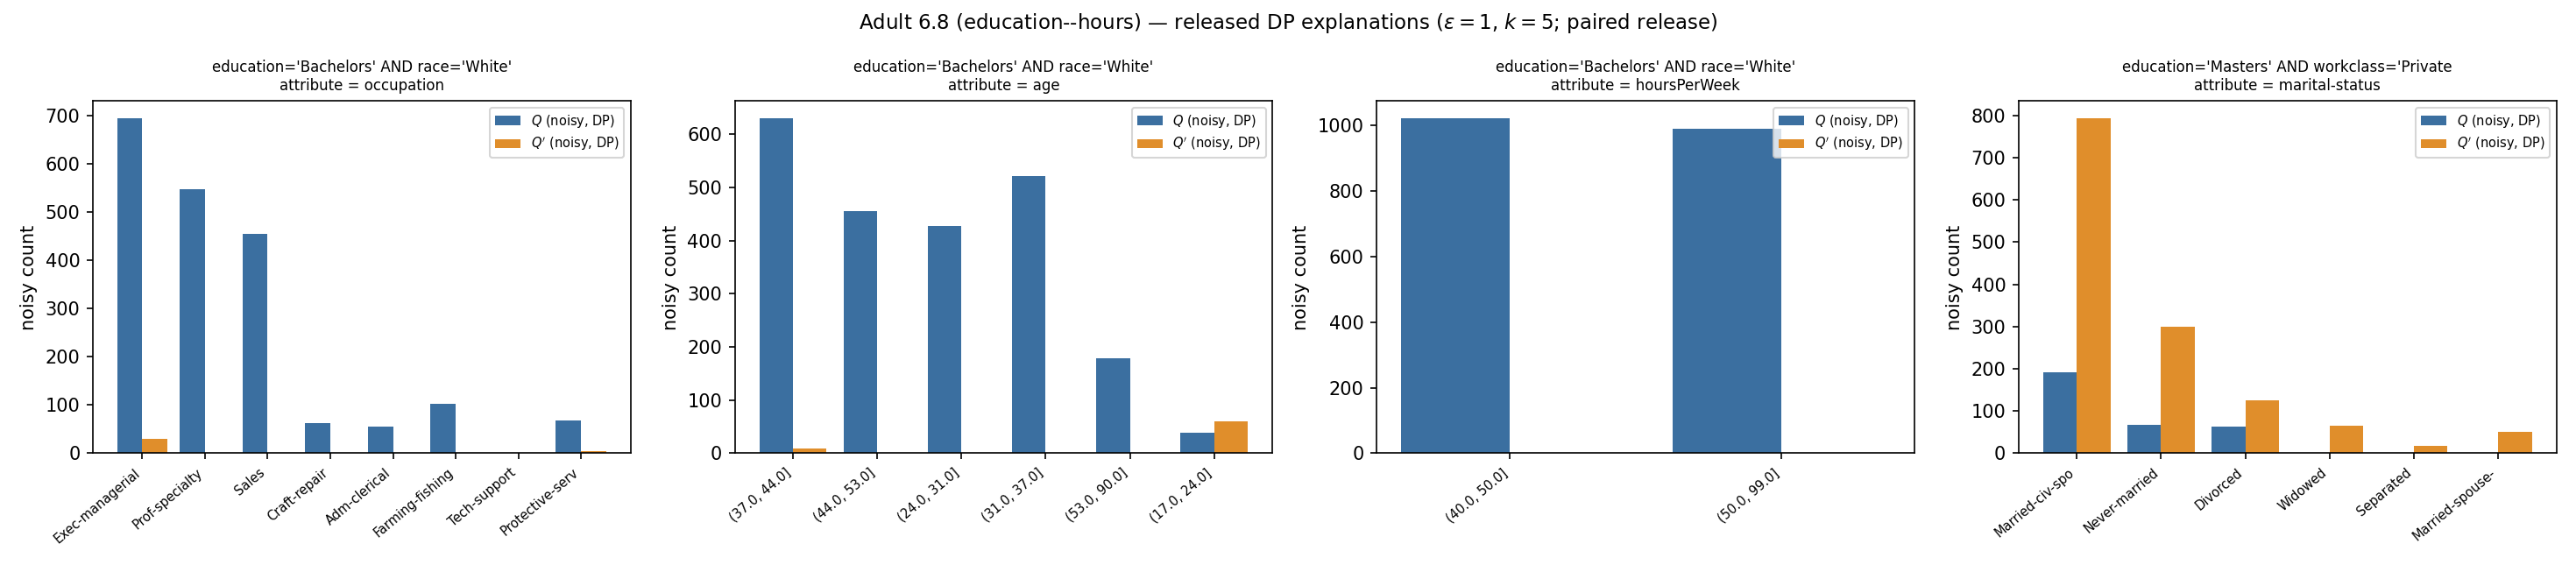
\includegraphics[width=\linewidth]{figures/U2_released_adult_education_hours.png}
\caption{A2: released $\epsilon=1$ explanations (paired release, two independently noised bars per bin). Blue is $Q$, orange is $Q'$.}
\label{fig:rel-adult-edu}
\end{figure*}
Three of the four panels are on \texttt{education='Bachelors' AND race='White'}, the population the refinement drops. Within it, the released counts say that the dropped workers are mostly executive-managerial, professional-specialty and sales workers, that they are spread over all age buckets from $24$ to $53$ and not concentrated in one, and that they are split about evenly between the 40--50 and 50+ hour buckets.
The fourth panel is on the people who come in. Within Masters degree holders in the private sector, $Q'$ adds mostly married-civilian-spouse people ($\approx790$ against $\approx190$ in $Q$), then never-married and divorced.

\paragraph{Bottom line.}
The refinement did not fix the representation of women by finding more women among the same kind of worker. It replaced a population of Bachelors-level managers and professionals working $50{+}$ hours with a smaller Masters-level population with a more married profile. That is a change in the kind of population, and the analyst may not want the second one. The constraint and the sizes alone cannot show this. In particular, the occupation panel tells the analyst that the high-income managerial concentration that motivated the original query has left the result.
\alon{Verify against the real histograms before submission: the figure is from a single run, the occupation claim reads off the first panel, and the claim about married people should be checked against the percentages of the female/male split inside that panel, since that is what links it to the constraint. If it does not link, drop the sentence.}

\subsubsection{Query refinement: removing a predicate on Tax (T1)}
\label{subsec:case-tax}

\paragraph{Scenario.}
An analyst studies low-rate taxpayers who are married: \texttt{MaritalStatus='M' AND Rate <= 5}.
A representation constraint requires at least $30\%$ of the result to have children (\texttt{HasChild='Y'}), and the result has only $3.5\%$.
ERICA~\cite{LMSJ23,ERICA} drops the marital-status predicate, and $Q'=\texttt{Rate <= 5}$ has $50.1\%$ \texttt{HasChild='Y'}.
The constraint is met with room to spare, and the analyst has to decide whether the result is still the group they meant to study.

\paragraph{What the user can see without our framework.}
The analyst can read two things off the queries: the result roughly doubled, and the share of taxpayers with children went from $3.5\%$ to $50.1\%$. The queries also say which predicate was removed, so the identity of the new population (single filers, among others) is not news. What the analyst cannot see is what the added taxpayers look like, and why the share of parents grew by more than a ``more people'' change would explain.

\paragraph{Stage 1: views.}
\alon{TODO: report how many of the $\tau=15$ retained views are conditioned on \texttt{MaritalStatus='S'}, and the rank of that view by $\Use$. This is the Tax counterpart of the ``Masters ranks 13th'' sentence in A2, and is not in the repository.}

\paragraph{Stage 2 and release.}
Figure~\ref{fig:rel-tax} shows the released explanations.
\begin{figure*}[t]
\centering
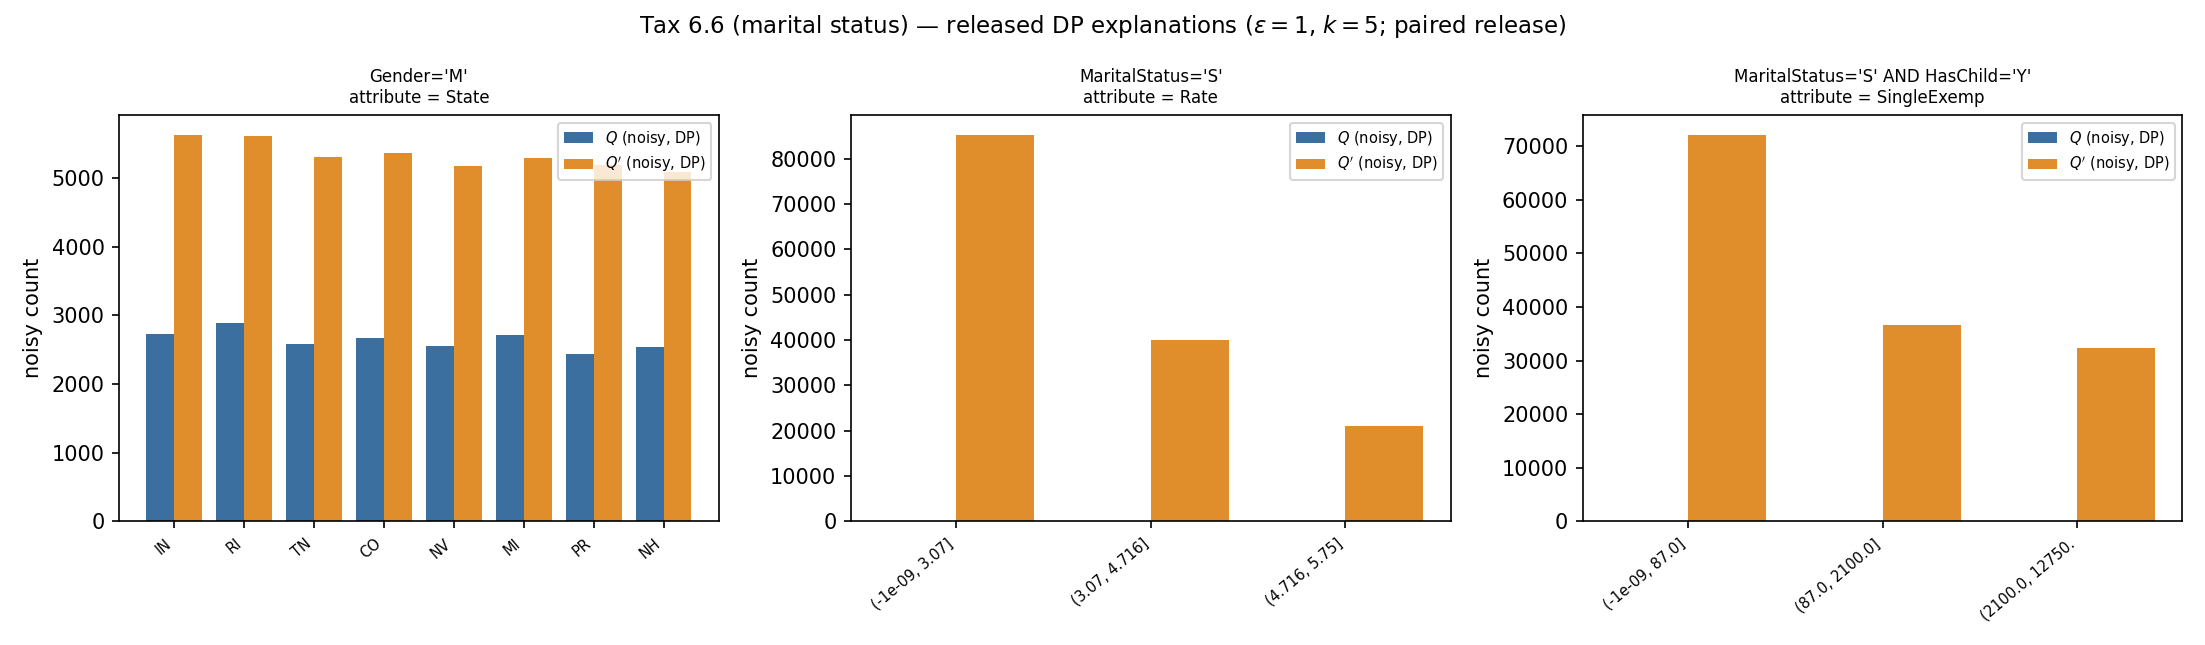
\includegraphics[width=\linewidth]{figures/U2_released_tax_marital.png}
\caption{T1: released $\epsilon=1$ explanations (paired release). Blue is $Q$, orange is $Q'$.}
\label{fig:rel-tax}
\end{figure*}
The first panel, on \texttt{Gender='M'}, shows $Q'$ at about twice $Q$ in every state, with no state standing out.
The other two panels are on single filers, the population the dropped predicate introduces ($Q$ contains none, by construction). The second shows that this added population sits at the bottom of the rate scale: about $85{,}000$ of the roughly $146{,}000$ added single filers fall in the lowest \texttt{Rate} bucket, and the counts fall in the two higher buckets.
The third panel is restricted to single filers \emph{with children}. Its three bins sum to about $140{,}000$, close to the whole added population, so nearly every single filer the refinement adds has a child.

\paragraph{Bottom line.}
The refinement is described as ``drop the marital-status filter'', but what it adds is not single filers in general. It is single parents, mostly with low rates. The constraint is satisfied because the added population is almost entirely the group the constraint asks for, not because the result became more balanced. An analyst who meant to keep studying a broad low-rate population learns that $Q'$ is a different group, and that its geographic profile is unchanged. That single filers appear without being told the predicate is something the analyst could have guessed; that they are mostly parents is not.
\alon{Verify before submission: the $\approx 96\%$ figure comes from adding the three bars of the third panel and dividing by the size of the added population, so it is read from noisy counts of a single run. Compute it from the exact (non-private) histograms for the text, and report the noisy value next to it so the reader sees the release preserves it. If the exact share is much lower, rewrite the bottom line.}

\subsubsection{Consistent query answering: Hospital (H1)}
\label{subsec:case-cqa}

\paragraph{Why CQA needs an explanation.}
A consistent answer keeps only the tuples that no repair removes. For a selection query on Hospital, these are the tuples of $Q(D)$ that take part in no violation of the three dependencies, which the conflict-hypergraph algorithm~\cite{chomicki2004} finds directly. The pair is $(Q(D),Q_\Sigma(D))$, and $Q_\Sigma(D)\subseteq Q(D)$ is the subpopulation the analyst is left with.
If the removed tuples were a random sample of $Q(D)$, this subpopulation would look like $Q(D)$ and the analyst could use it as is. If they are not (for example because errors are concentrated in some cities, ownership types or services), then aggregates over $Q_\Sigma(D)$ describe a different population from the one the query asked about.
This is the same question as in query refinement, asking what kind of tuples the change took out or brought in, with one difference: $Q$ is not edited by anyone, so there is no changed predicate to read the answer from. The analyst sees only the sizes $|Q(D)|$ and $|Q_\Sigma(D)|$.

\paragraph{How we chose the pair.}
We take single-predicate selection queries on attributes that describe a hospital and compute $Q_\Sigma$ for each with the algorithm above. We keep a query only when $Q_\Sigma$ removes a visible but not complete share of $Q$, so that there is something to explain and something left to compare against. H1 is the selection \texttt{HospitalType='Acute Care Hospitals'}; H2 and H3 follow the same rule on \texttt{EmergencyService} and \texttt{HospitalOwner} (Table~\ref{tab:query-pairs}).

\paragraph{What the user can see without our framework.}
The two sizes, and the identity of the three dependencies.

\paragraph{Release and bottom line.}
\alon{TODO: run H1--H3. For each, report $|Q|$, $|Q_\Sigma|$, the retained views and the released histograms, and one sentence on which part of the answer the repair changed and whether it did so evenly, which is the point of the case.}

% ---------------------------------------------------------------
\subsection{Accuracy and Performance Analysis}
\label{subsec:exp-analysis}

\subsubsection{Accuracy}
\label{subsec:quality}

\begin{table}[t]
\centering
\small
\caption{ApproxRatio against each baseline, $\epsilon=1$ and $\epsilon=5$, $40$ trials.}
\label{tab:quality}
\begin{tabular}{@{}lcccccc@{}}
\toprule
& \multicolumn{3}{c}{$\epsilon=1$} & \multicolumn{3}{c}{$\epsilon=5$}\\
\cmidrule(lr){2-4}\cmidrule(lr){5-7}
Pair & \Bone & \Btwo & \Bthree & \Bone & \Btwo & \Bthree\\
\midrule
A1 & 0.883 & 0.875 & 0.875 & 0.950 & 0.941 & 0.941\\
A2 & 0.691 & 0.612 & 0.612 & 0.950 & 0.842 & 0.842\\
T1 & 0.931 & 0.901 & 0.901 & 0.995 & 0.963 & 0.963\\
\bottomrule
\end{tabular}
\end{table}

\begin{figure*}[t]
\centering
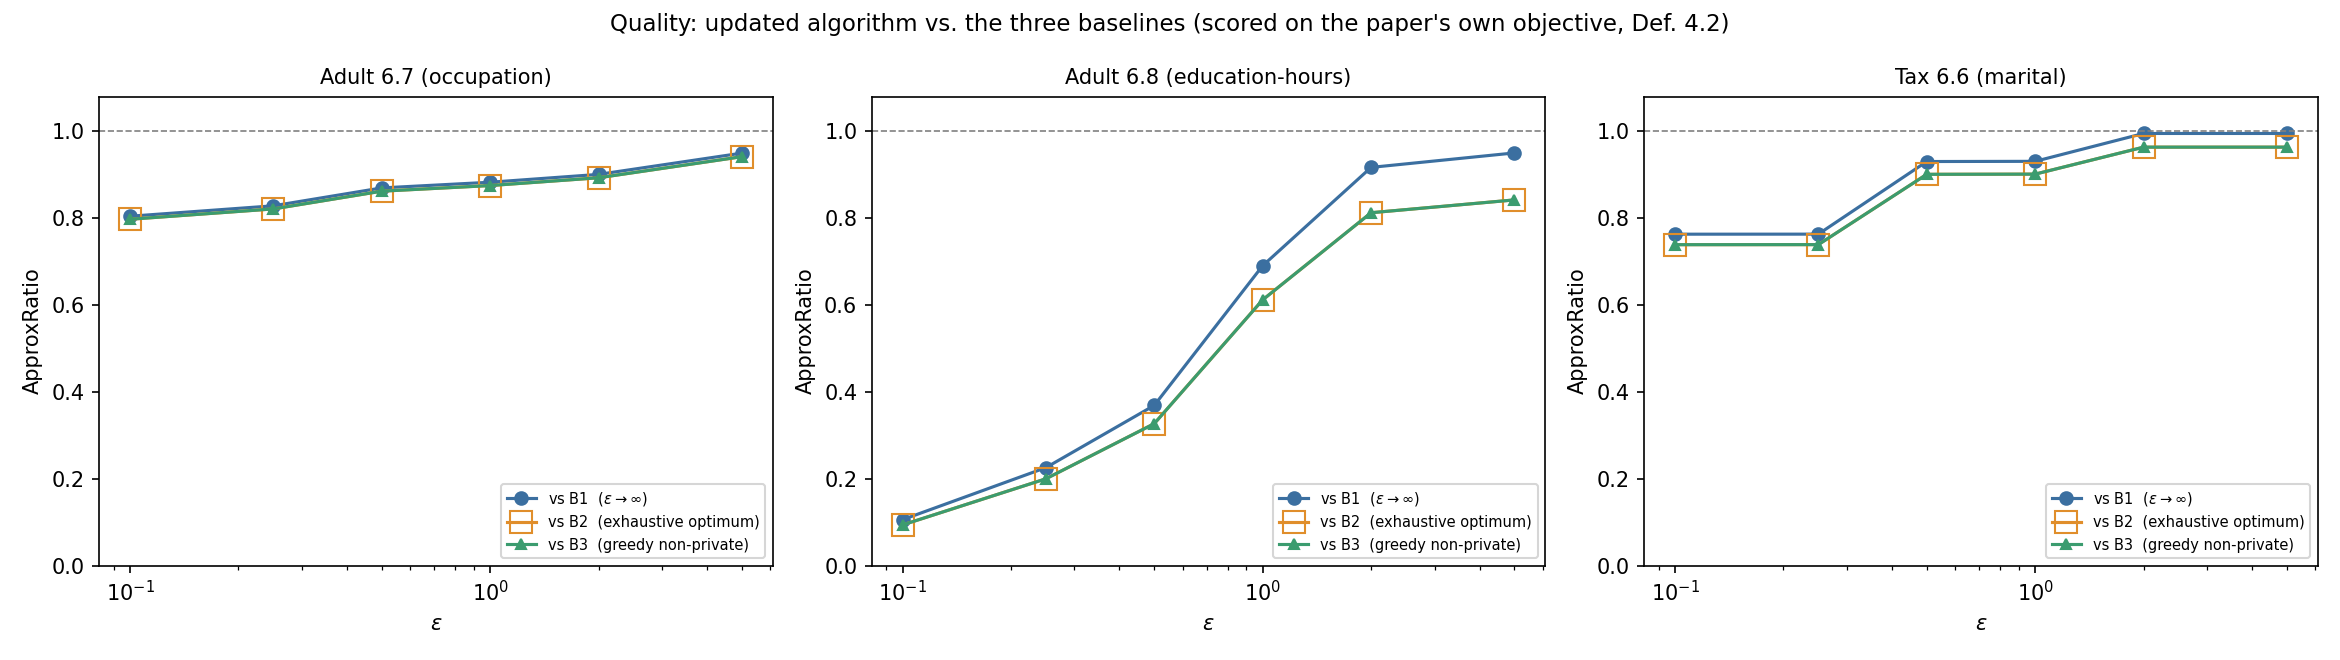
\includegraphics[width=\linewidth]{figures/Q1_approxratio_vs_baselines.png}
\caption{ApproxRatio against each baseline as a function of $\epsilon$ (measured with $\gamma_{\mathrm{eval}}=0$).}
\label{fig:quality}
\end{figure*}

At the default budget the released set reaches $0.88$--$0.93$ of the noise-free score on A1 and T1 and $0.88$--$0.90$ of the exhaustive optimum (Table~\ref{tab:quality}). Three observations follow from the data.

\paragraph{A pair is hard when its candidates are close, not when it is small.}
A2 has the lowest ratio ($0.69$ against \Bone{} at $\epsilon=1$, $0.11$ at $\epsilon=0.1$), while T1, with ten times the data, has the highest. The exponential mechanism separates two candidates only if their utilities differ by more than about $2\,\Delta u\ln|C|/\epsilon_S$. On A2 the gap between the leading candidates (the \emph{margin}) is $0.027$, against $0.121$ on A1 and $0.315$ on T1, so the mechanism has little to separate. The margin, not $N$, tracks the difficulty, and it is a property of the query pair rather than of the data size.

\paragraph{Greedy matches the optimum, so the private gap comes from privacy alone.}
\Btwo{} and \Bthree{} coincide to the last digit on all three pairs, as Proposition~\ref{prop:greedy-exact} predicts. So the remaining gap to \Bthree{} cannot be due to the greedy order of selection; it comes from noise and from the private view filter. The ratio to \Btwo/\Bthree{} sits below the ratio to \Bone{} by $0.01$--$0.11$, and that difference is the cost of filtering views privately. It is largest on A2, which fits the budget-split observation in Section~\ref{subsec:exp-setup}, that the view stage cannot be given less budget.
\alon{TODO (experiment to add): the view stage in isolation. For each pair and $\epsilon_P$, the overlap of the privately retained $\tau$ views with the exact top-$\tau$ by $\Use$, and the lowest $\Use$ retained against the true $\tau$-th best. A first look at A2 suggests the overlap is low at the budgets used here and rises sharply with $\epsilon_P$, which would be the direct evidence for the claim above.}

\paragraph{Smoothing has to be matched to the bins, not to $N$.}
$\gamma$ competes with the size of individual histogram bins, and these differ much more than $N$ does: the median non-empty bin holds $20$ tuples on Adult and $3{,}897$ on Tax, a factor of $200$ for a factor of $10$ in $N$. With $\gamma$ at $0.5\%$ of $N$, it exceeds the bin count for $84\%$ of Adult bins but $30\%$ of Tax bins, and at $5\%$ of $N$ it exceeds $98\%$ and $94\%$, where $\HD_\gamma$ no longer measures relative change. The margins above imply a required $\gamma$ of about $292$, $66$ and $25$ for A2, A1 and T1, which is the reverse of the order of dataset size. This is why $\gamma$ is derived from $\tau$, $|\Attrs|$ and the budget (Eq.~\eqref{eq:gamma-rule}) and not from $N$.
\alon{Re-check this paragraph after the rerun: it was measured under the old $\gamma$ rule and may be partly superseded.}

\subsubsection{Performance}
\label{subsec:scalability}

\begin{figure*}[t]
\centering
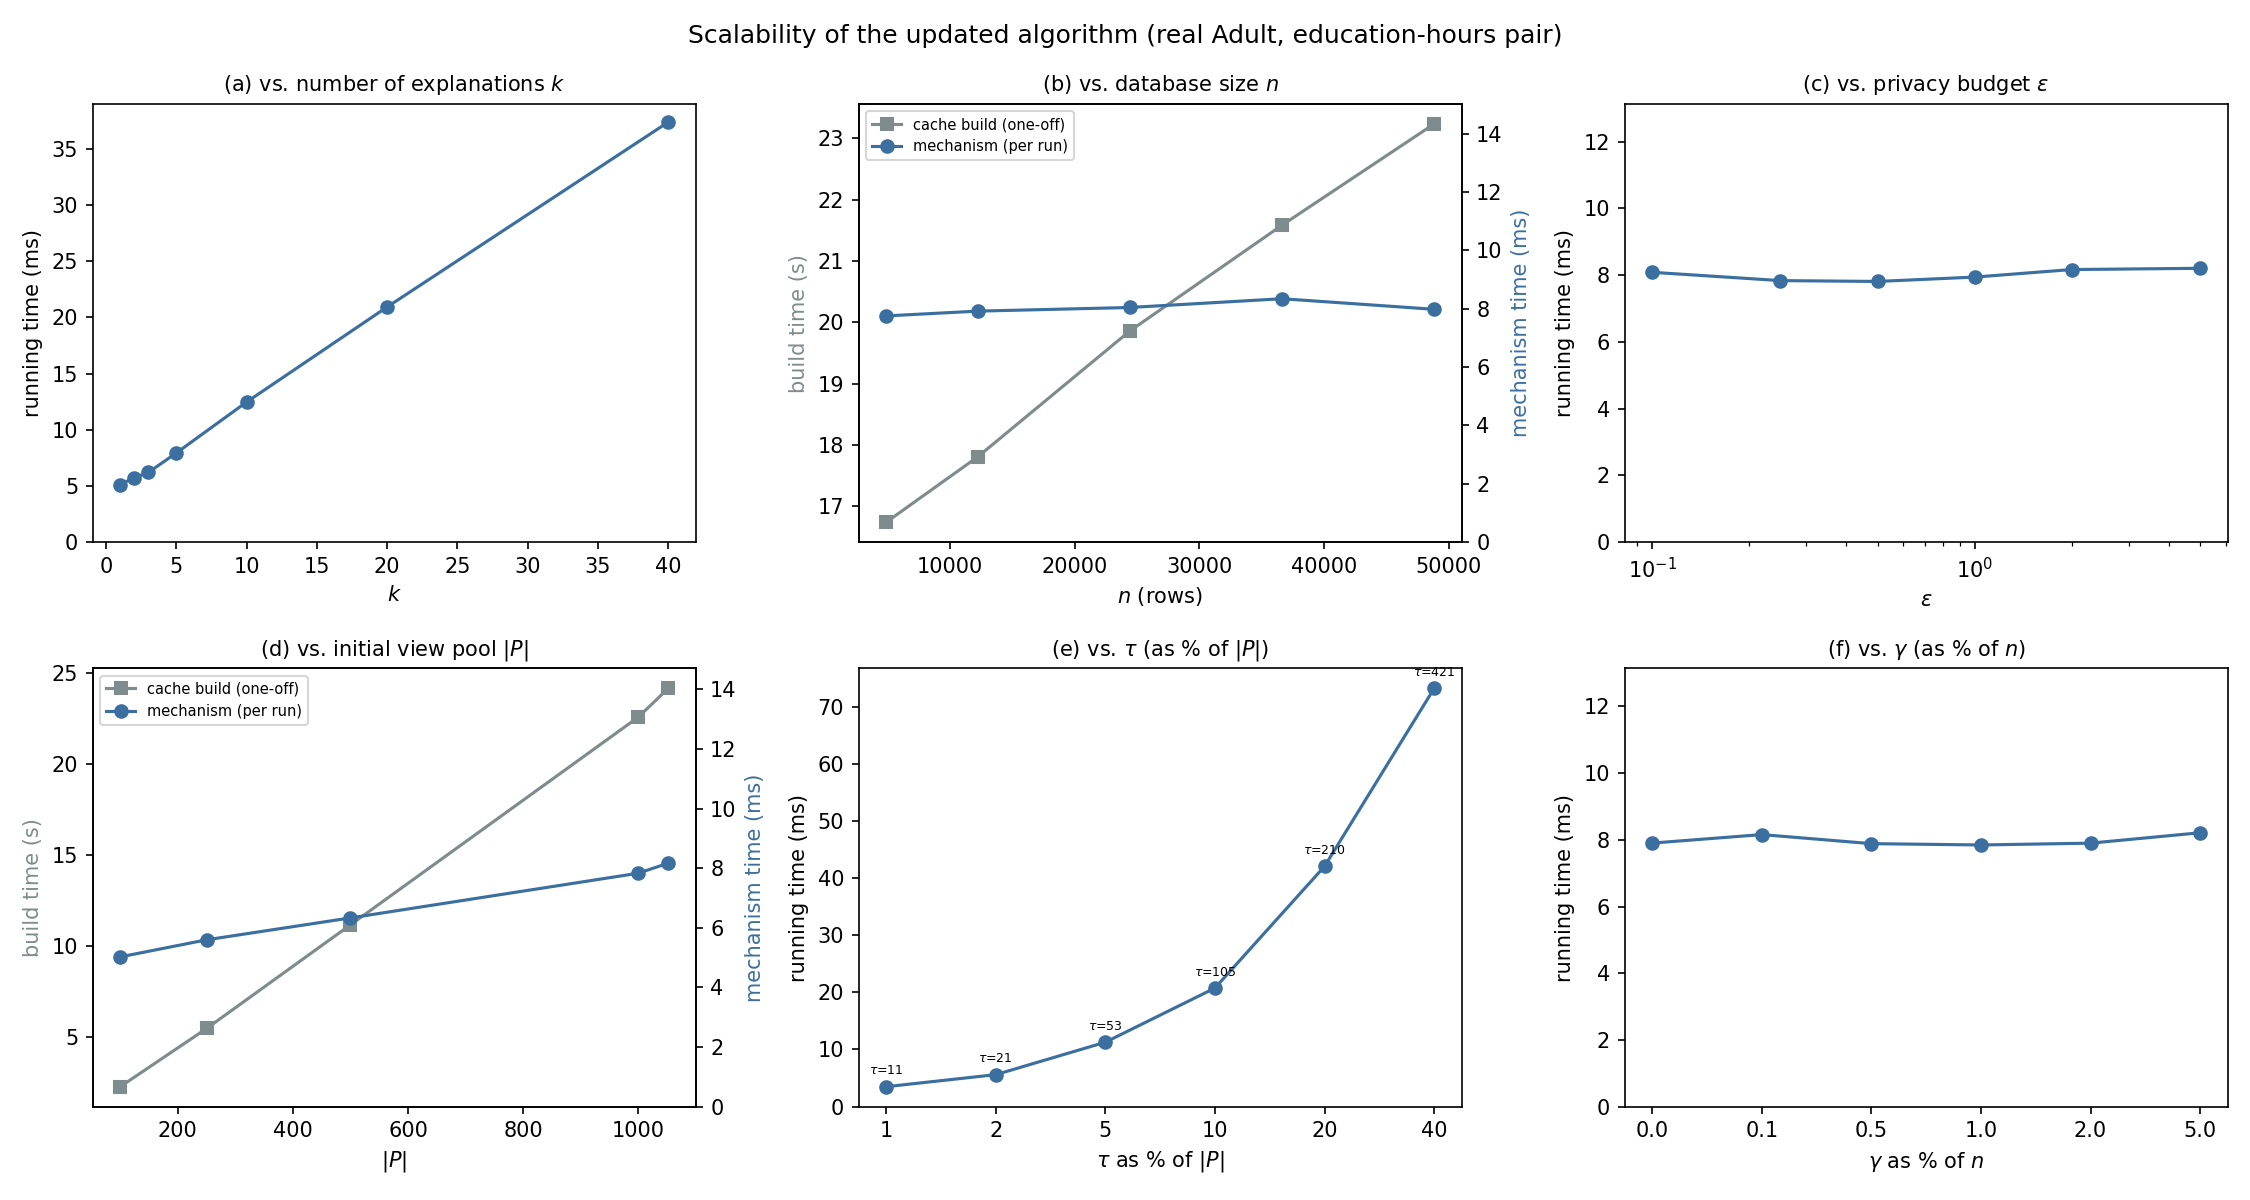
\includegraphics[width=\linewidth]{figures/S1_scalability_grid.png}
\caption{Running time of the algorithm. Panels (b) and (d) separate the one-off cache build from the per-invocation cost.}
\label{fig:scalability}
\end{figure*}

The per-invocation cost is linear in $k$ ($4.6$\,ms at $k=1$ to $36.3$\,ms at $k=40$) and in $\tau$, and flat in $N$ ($7.7$--$8.3$\,ms over a tenfold range). This follows from the structure in Section~\ref{subsec:complexity-analysis}: all the $O(N)$ work is in the one-off preprocessing ($16.7$\,s rising to $23.2$\,s over the same range), and the $k$ selection rounds only touch the $\tau|\Attrs|$ cached scores. The same cache lets $\gamma$ change at no cost, and the running time does not depend on $\epsilon$ ($7.8$--$8.2$\,ms for $\epsilon\in[0.1,5]$), so a user can re-run at a different budget interactively.

\begin{figure}[t]
\centering
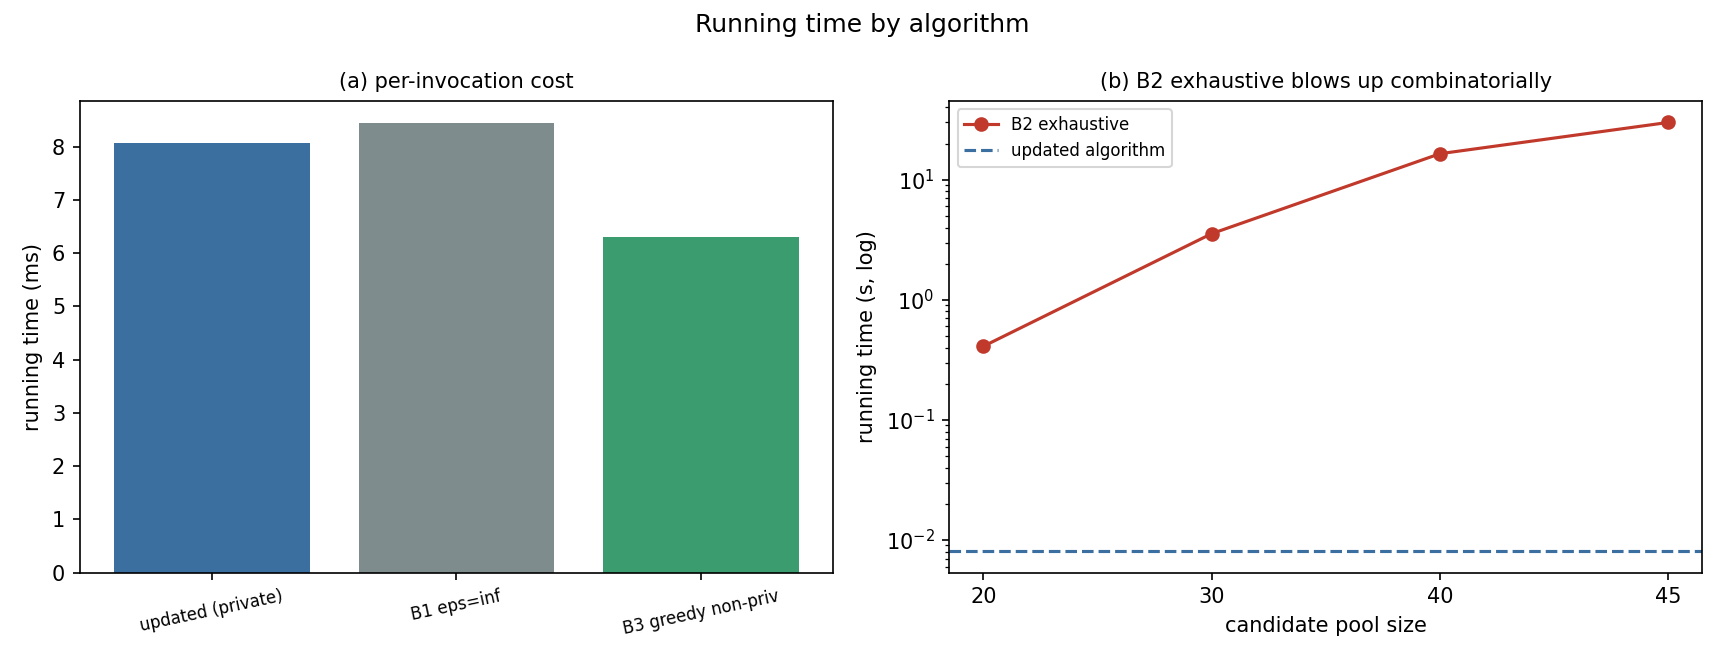
\includegraphics[width=\linewidth]{figures/S2_runtime_by_algorithm.png}
\caption{Per-invocation cost of each method, and the growth of \Btwo.}
\label{fig:runtime-algorithm}
\end{figure}

Privacy adds little running time: the private algorithm takes $8.1$\,ms, \Bone{} $8.4$\,ms and \Bthree{} $6.3$\,ms. The exponential mechanism replaces an $\arg\max$ over the same scores. \Btwo{} is different in kind: it grows from $0.41$\,s at $20$ candidates to $30$\,s at $45$, a $73\times$ increase for a $2.25\times$ larger pool, and takes $57$\,s on the $50$-candidate pool. The private algorithm returns a set of the quality the exhaustive search gives, up to the privacy gap above, about four orders of magnitude faster.
\alon{TODO: runtime of the CQA and StackOverflow pairs, and an end-to-end time including the one-off cache build per pair, for the table.}
